\section{Experiment}
\label{exp_appendix}
\subsection{$\beta$-DPO Implementation Details and Hyperparameters}
\label{setup_exp}
$\beta$-DPO is relatively straightfoward to implement; The full algorithm is summarized in Algorithm \ref{alg}.
% The  for the $\beta$-DPO loss is provided below:

\begin{algorithm}[h]
    \caption{$\beta$-Direct Preference Optimization}\label{alg:beta-dpo}
    \begin{algorithmic}[1]
    \REQUIRE Preference dataset $\mathcal{D}$, batch size $b$, constraint coefficient $\beta_0$, selection ratio $\rho$, scaling factor $\alpha$, and learning rate $\eta$.
    \STATE Initialize model $\pi_{\theta_0}$ with supervised finetuning on $\mathcal{D}$.
    % \FOR{$n=1\ldots N$ iterations}
    \WHILE{not converged}
        \STATE Sample a batch $\mathcal{B} = \{(\xb^{(i)}, \yb_w^{(i)}, \yb_l^{(i)})\}_{i=1}^b$ from $\mathcal{D}$.
        \STATE Compute the individual reward discrepancy $M_i = r(\yb_w^{(i)};\xb^{(i)})-r(\yb_l^{(i)};\xb^{(i)})$.
        \STATE Update the threshold $M_0$ and $\sigma$ using Equations \eqref{mom} and \eqref{mom2}.
        \STATE Sample $b \times \rho$ samples without replacement based on $p(M_i)$ in Equation \eqref{sampling_p}.
        \STATE Compute the batch-level $\beta$ using Equation~\eqref{eq:beta}.
        \STATE Compute the loss using the Equation~\eqref{eq:DPO2}.
        \STATE Compute the gradient and update the model $\theta_t \leftarrow \theta_{t-1} - \eta \nabla_\theta  \ell(\theta_{t-1}, \mathcal{B})$.
    \ENDWHILE
    % \ENDFOR
\RETURN Final model $\pi_{\theta}$.
\end{algorithmic}
\label{alg}
\end{algorithm}

Unless noted otherwise, we use a $\beta=0.1$, batch size of 64, $m=0.9$ to ensure the stability of the global $M_i$ estimation, $\rho=0.8$ to filter 20\% uninformative samples, and the Adam optimizer with a learning rate $5e-7$ by default.  We carried out all computational tasks on a suite of four 80GB A100 GPUs. For the Pythia-410M model, we use a batch size of 128, while the rest of the parameters remain the same.

% In paticular, for \textbf{single-turn dialugue} , we utilize \textbf{Pythia-2.8, -1.4b and -410M} to conduct the experiments on Anthropic-HH dataset. In this setting, no pre-trained SFT model is available; we therefore fine-tune an off-the-shelf language model on the only the preferred completions to form the SFT model. As for \textbf{summarization}, we use the Reddit TL;DR summarization dataset along with human preferences gatherd by \citet{tldr2}. We use an SFT model fine-tuned on human-written forum post summaries \footnote{https://huggingface.co/CarperAI/openai_summarize_tldr_sft} with the TRLX \cite{havrilla-etal-2023-trlx} framework for RLHF. The human preference dataset was gathered by \citet{tldr2} on samples from a different, but similarly-trained, SFT model.

In examining the arena of \textbf{single-turn dialogue}, our experimental framework leverages Pythia-2.8, Pythia-1.4b, and Pythia-410M for empirical analysis using the Anthropic-HH dataset. Given the absence of a pre-existing Supervised Fine-Tuning (SFT) model tailored for this dataset, we fine-tune an accessible language model exclusively with preferred completions to sculpt our SFT model.
Turning our focus to the domain of \textbf{summarization}, we employed the Reddit TL;DR summarization dataset, enriching our research with human preferences as documented by the study \cite{tldr2}. Our methodology here incorporates an SFT model meticulously fine-tuned on expert-composed summaries of forum posts \footnote{\url{https://huggingface.co/CarperAI/openai_summarize_tldr_sft}}, operating within the TRLX framework for Reinforcement Learning from Human Feedback (RLHF), as introduced by \citet{havrilla-etal-2023-trlx}. The human preference dataset was gathered by \citet{tldr2} on samples from a different, but similarly-trained, SFT model.
\subsection{Mixture of \emph{low gap} and \emph{high gap}}
\label{low_gap_high_gap}

In our previous discussion, we identified a \emph{low gap} dataset, constituted by pairs of responses generated from the HH dataset. Given that these responses originate from the same model, we can infer that they represent semantically similar answers, hence the designation \emph{low gap}. Concurrently, we maintain the positive samples constant while selecting negative samples generated by a Pythia 2.8B model. The significant performance disparity between the models results in a considerable variation in the quality of these negative samples, which we refer to as the \emph{high gap}. We mix these two types of data in varying proportions to mimic the distribution of data in real-world scenarios. We label this approach the "mixture experiment." To facilitate a better comparison of the distributions across different ratios, we proceed to illustrate our findings with the following graph:

\begin{figure}[t]
    \vspace{-10pt}
    \centering
    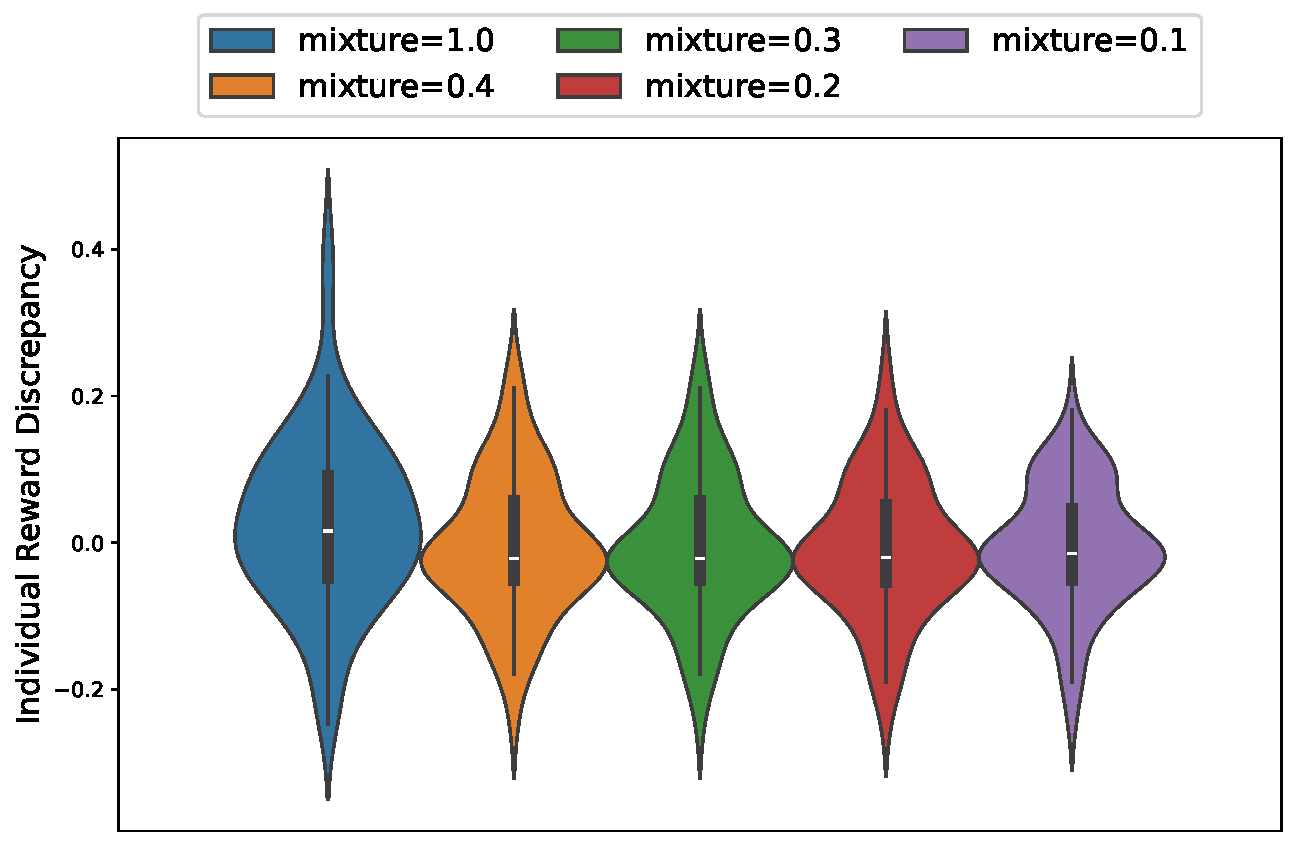
\includegraphics[width=0.6\linewidth]{figs/gap_mixture2.pdf}
    % \vspace{-10pt}
    \caption{
        Distribution of individual reward discrepancies following the Pythia-2.8B model.
    }
    \label{fig_mix}
    % \vspace{-10pt}
\end{figure}
Figure \ref{fig_mix} clearly illustrates that as the mixture ratio increases—that is, the proportion of high gap data rises—the dispersion of the overall dataset broadens. Conversely, a decrease in the mixture ratio, corresponding to an elevated presence of low gap data, results in a more concentrated distribution of reward discrepancy.
% \subsection{$\beta$-DPO and KTO, SPPO}

\begin{figure}[t]
    \vspace{-10pt}
    \centering
    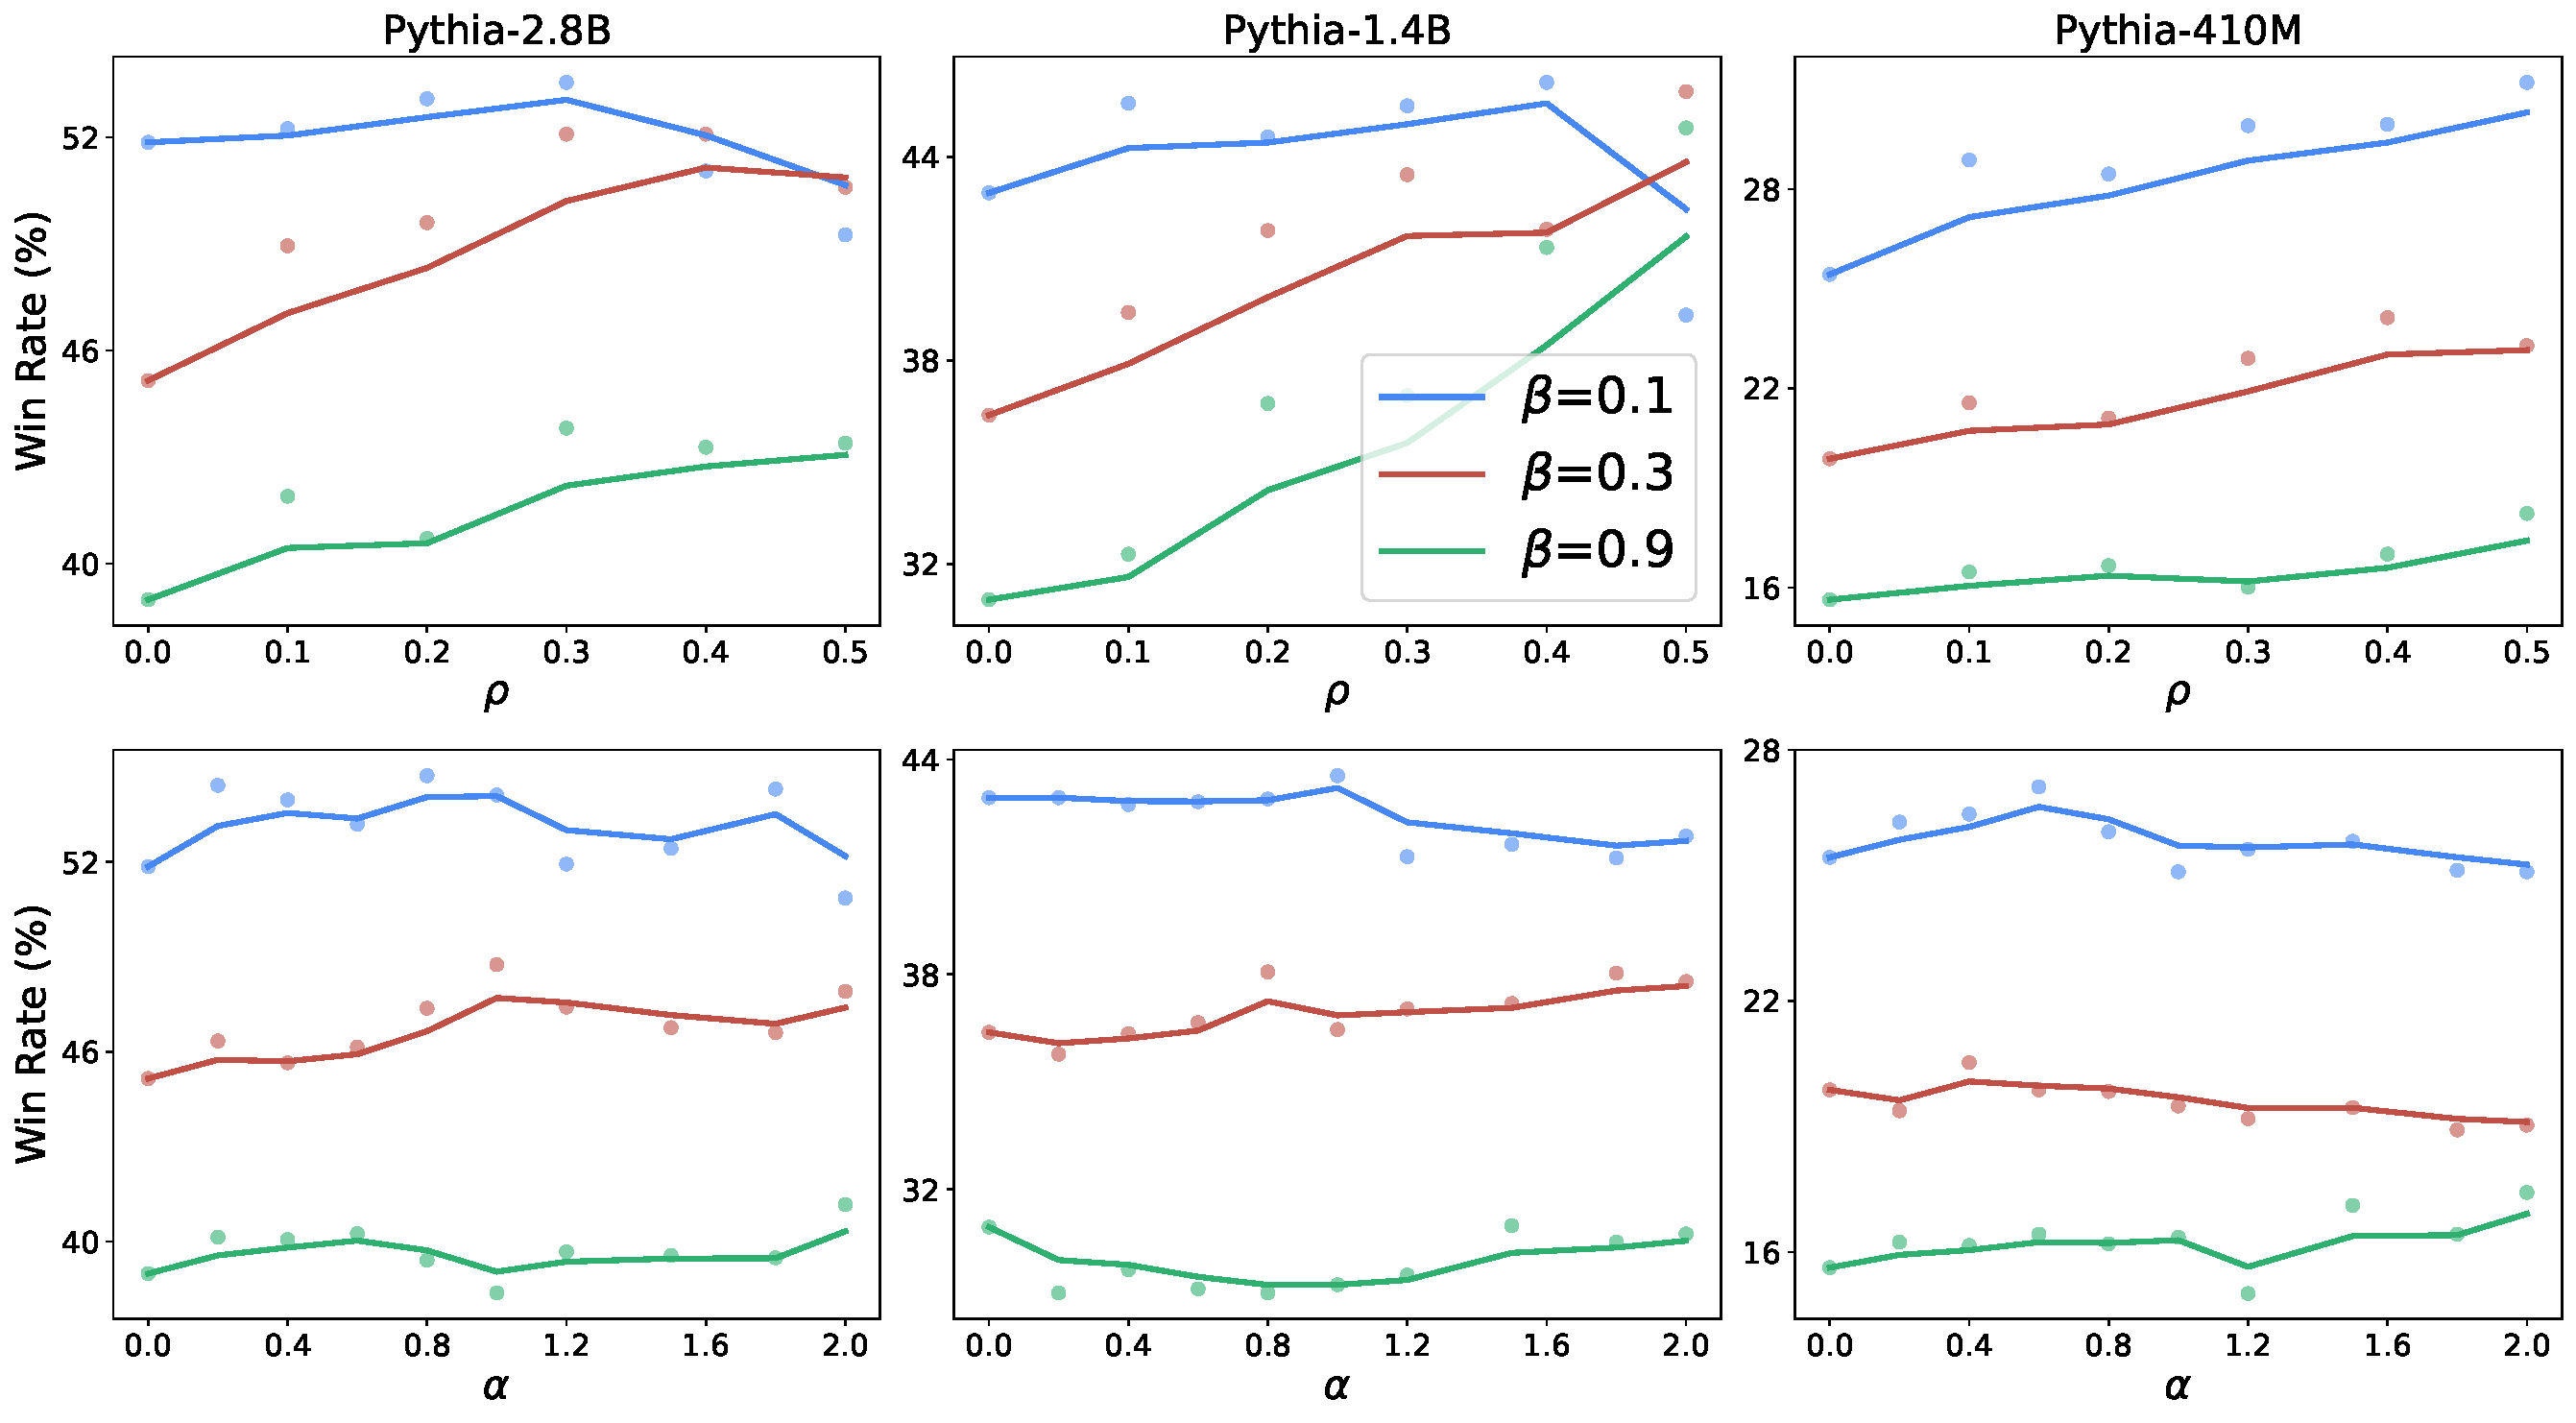
\includegraphics[width=0.8\linewidth]{figs/params_beta_DPO.pdf}
    % \vspace{-10pt}
    \caption{
        Performance comparison across different $\beta$ values and $\rho$ values for three different model sizes (Pythia-2.8B, Pythia-1.4B, and Pythia-410M) on the Anthropic HH dataset using GPT-4 as the evaluator. Each subplot represents the win rate for varying parameters $\beta$ = 0.1, 0.3, and 0.9 with exponential smoothing.
    }
    \label{fig_params}
    \vspace{-10pt}
\end{figure}

\subsection{Hyperparameter Sensitivity}
In this section, we investigate the impact of key hyperparameters in the $\beta$-DPO methodology, using the Anthropic HH dataset and leveraging models such as Pythia-2.8B and GPT-4 for evaluation. Specifically, we examine the influence of varying the hyperparameters $\alpha$ and the filtering ratio $\rho$. The parameter $\alpha$ is explored across a broad spectrum of values including $0.2$, $0.4$, $0.6$, $0.8$, $1.0$, $1.2$, $1.5$, $1.8$, and $2.0$. Concurrently, the filtering ratio $\rho$ is investigated at intervals ranging from $0.1$ to $0.5$, at a granularity of $0.1$. This comprehensive analysis aims to unravel how these hyperparameters affect the performance and outcomes of the $\beta$-DPO process.

\textbf{Static $\beta$ vs. Dynamic $\beta$.}
Our results, as depicted in Figure \ref{fig_params}, reveal that a dynamic $\beta$ (where $\alpha \neq 0$) prevails over a static $\beta$ (where $\alpha = 0$) under an exhaustive range of hyperparameter configurations. 
This outcome aligns seamlessly with our underlying premise: static beta fails to fully leverage a model's potential when confronted with varying data quality within a dataset. Furthermore, our observations highlight an intriguing trend: as $\alpha$ increases, the performance of the $\beta$-DPO model initially improves before declining, typically peaking within the interval of 0.6 to 1.0. 

\textbf{Filtering Ratio $\rho$ Sensitivity.}
As illustrated in the figure \ref{fig_params}, varying model sizes exhibit distinct sensitivities to the parameter $\rho$. Within the context of the Pythia-2.8B model, a $\rho$ value of 0.3 yields optimal performance, whereas for the Pythia-410M model, a $\rho$ value of 0.5 is superior. This can be posited to suggest that smaller models may require more stringent data filtering to perform optimally, whereas larger models possess the increased capacity necessary for learning the most effective strategies. This insight provides a significant directive for future research: the value of $\rho$ should be fine-tuned according to the specific circumstances of the application.


\subsection{The ablation study \wrt $M_0$}
In this work, we employed a moving average updating scheme \cite{mae} for the updating of $M_0$. In order to investigate the superiority of this configuration, we also conducted a comparative experiment involving hyperparameter settings. Specifically, $M_0$ was treated as a constant in the training process, while all other settings remained unchanged. The experimental results are as follows:
\begin{table}[h]
    \centering
    \caption{
    Comparison of win rates across varying $M_0$ in $\beta$-DPO.
    }
    \begin{tabular}{l|l|l|l|l|l|l|l}
        \toprule
        \textbf{$M_0$} & 0 & 1 & 3 & 5& 7& 10 & Moving Average\\
        \midrule
        $\beta$-DPO & $53.35$ & $54.00$ & $53.85$ & $55.61$  &$53.19$ & $56.75$& $57.07$ \\
        \bottomrule
    \end{tabular}
    \label{tab:constant_m0}
\end{table}

As demonstrated in Table \ref{tab:constant_m0}, by tuning $M_0$, we were able to achieve significant performance improvements, which approached the performance level of the moving average updating scheme. This clearly underscores the superiority of the moving average updating scheme. On one hand, it obviates the need for an additional manual search process. On the other hand, it facilitates stable performance enhancements.

\subsection{Our Methods with Explicit Reward Model}
\label{sec:appendix_explicit_rm}
To broaden the application of the $\beta$-DPO strategy for alignment and to address the limitations of DPO's implicit reward model, we incorporated two external reward models (RMs):

\begin{itemize}[leftmargin=*]
    \item We utilized \href{https://huggingface.co/llm-blender/PairRM}{llm-blender/PairRM}~\cite{Jiang2023LLMBlenderEL} to score the chosen and rejected responses, denoted as \(r_{w,\text{PairRM}}, r_{l,\text{PairRM}}\).
    \item We adopted the v0.2 Llama3-Instruct setting \cite{SimPO2024} by employing \href{https://huggingface.co/RLHFlow/ArmoRM-Llama3-8B-v0.1}{{RLHFlow/ArmoRM-Llama3-8B-v0.1}}~\cite{ArmoRM} as the reward model to rank responses, denoted as \(r_{w,\text{ArmoRM}}, r_{l,\text{ArmoRM}}\).
\end{itemize}

{The other algorithmic processes (refer to Appendix Algorithm~\ref{alg:beta-dpo}) remain unchanged, with modifications made only to \(M_{i,\text{PairRM}}=r_{w,\text{PairRM}}^{(i)} - r_{l,\text{PairRM}}^{(i)}\) and \(M_{i,\text{ArmoRM}}=r_{w,\text{ArmoRM}}^{(i)} - r_{l,\text{ArmoRM}}^{(i)}\).} 
For comparison with baselines, we assess our models using one of the most popular open-ended instruction-following benchmarks: AlpacaEval 2.
% We tested the implicit reward model on the state-of-the-art loss function (SimPO \cite{SimPO2024}). 
The detailed results are as follows:

\begin{table}[h]
\centering
\caption{Comparison of different methods on Llama3-Instruct (8B) with explicit reward model}
\begin{tabular}{lcc}
\toprule
\textbf{Method} & \textbf{Llama3-Instruct (8B)} & \textbf{Llama3-Instruct (8B)} \\
\midrule
 & \textbf{LC (\%)} & \textbf{WR (\%)} \\
\midrule
DPO (Implicit RM) & 40.44 & 37.38 \\
$\beta$-DPO (Implicit RM) & \textbf{43.38} & \textbf{38.21} \\
\midrule
SimPO (Implicit RM) & 44.38 & 38.97 \\
$\beta$-SimPO (Implicit RM) & \textbf{46.03} & \textbf{40.18} \\
\midrule
SimPO (PairRM) & 44.70 & 38.98 \\
$\beta$-SimPO (PairRM, Instance-Level) & 43.84 & 38.54 \\
$\beta$-SimPO (PairRM, Batch-Level) & \textbf{45.65} & \textbf{39.76} \\
\midrule
SimPO (ArmoRM) & 53.70 & 47.50 \\
$\beta$-SimPO (ArmoRM, Instance-Level) & 49.05 & 45.47 \\
$\beta$-SimPO (ArmoRM, Batch-Level) & \textbf{54.86} & \textbf{49.66} \\
\bottomrule
\end{tabular}
\label{tab:comparison}
\end{table}

From the results above, we observed the following:

\textbf{The proposed dynamic $\beta$ strategy demonstrates strong generalizability.} Both $\beta$-{D,Sim}PO consistently yield stable performance improvements across implicit and explicit RMs.

\textbf{Batch-level performance is crucial.} In explicit RM settings, batch-level dynamic $\beta$ consistently outperforms instance-level dynamic $\beta$.

\subsection{GPT-4 prompts for computing summarization and dialogue win rates}
\label{app:prompts}
A fundamental element of our experimental framework involves the assessment of win rates facilitated by GPT-4. In this segment, we delineate the prompts employed to ascertain win rates pertinent to our summarization and dialogue-oriented investigations. For the entirety of our experimental endeavors, we utilize GPT-4. It is important to note that the sequence in which summaries or responses are presented is randomized for each evaluation.
% A key component of our experimental setup is GPT-4 win rate judgments. In this section, we include the prompts used to generate win rates for the summarization and dialogue experiments. We use \texttt{gpt-4} for all our experiments. The order of summaries or responses are randomly chosen for every evaluation.
\\[2mm]
\textbf{Summarization GPT-4 win rate prompt.}
\begin{verbatim}
Which of the following summaries does a better job of summarizing the most \
important points in the given forum post?

Post:
<post>

Summary A:
<Summary A>

Summary B:
<Summary B>

FIRST provide a one-sentence comparison of the two summaries, explaining which \
you prefer and why. SECOND, on a new line, state only "A" or "B" to indicate your \ 
choice. Your response should use the format:
Comparison: <one-sentence comparison and explanation>
Preferred: <"A" or "B">
\end{verbatim}

\textbf{Dialogue GPT-4 win rate prompt.}
\begin{verbatim}
For the following query to a chatbot, which response is more helpful?

Query: <the user query>

Response A:
<either the test method or baseline>

Response B:
<the other response>

FIRST provide a one-sentence comparison of the two responses and explain \
which you feel is more helpful. SECOND, on a new line, state only "A" or \
"B" to indicate which response is more helpful. Your response should use \
the format:
Comparison: <one-sentence comparison and explanation>
More helpful: <"A" or "B">
\end{verbatim}

\section{Broader Impacts}
\label{broader_impacts}
This paper presents work whose goal is to advance the field of Machine Learning. There are many potential societal consequences of our work, none of which we feel must be specifically highlighted here.